\documentclass[12pt, titlepage]{article}

\usepackage{booktabs}
\usepackage{tabularx}
\usepackage{hyperref}
\hypersetup{
    colorlinks,
    citecolor=black,
    filecolor=black,
    linkcolor=red,
    urlcolor=blue
}
\usepackage[round]{natbib}

\usepackage{amsmath, amsfonts}
\usepackage[margin=1in]{geometry}
\usepackage{amssymb}
\usepackage{amsthm}
\usepackage{amsmath}
\usepackage{multirow}
\usepackage{verbatim}
\usepackage{listings}
\usepackage{color}
\usepackage{hyperref}
\usepackage{blindtext}
\usepackage{cancel}
\usepackage{float}
\usepackage{enumitem}
\usepackage{graphicx}
\usepackage{makecell}

\usepackage[table]{xcolor}
\setlength{\tabcolsep}{18pt}
\renewcommand{\arraystretch}{1.5}
\renewcommand{\labelenumi}{\theenumi.}
\renewcommand{\labelenumii}{\theenumii.}
\renewcommand{\labelenumiii}{\theenumiii.}
\newcommand{\be}{\begin{enumerate}}
\newcommand{\ee}{\end{enumerate}}
\newcommand{\bi}{\begin{itemize}}
\newcommand{\ei}{\end{itemize}}
\newcommand{\bc}{\begin{center}}
\newcommand{\ec}{\end{center}}
\newcommand{\bv}{\begin{verbatim}}
\newcommand{\ev}{\end{verbatim}}
\newcommand{\ba}{\begin{align*}}
\newcommand{\ea}{\end{align*}}
\newcommand{\beq}{\begin{equation*}}
\newcommand{\eeq}{\end{equation*}}
\newcommand{\bs}{\begin{split}}
\newcommand{\es}{\end{split}}
\newcommand{\mname}[1]{\mbox{\sf #1}}
\newcommand{\pnote}[1]{{\langle \text{#1} \rangle}}
\renewcommand{\labelenumii}{\theenumii.}


\title{Software Requirements Specification\\ASLingo Application}

\author{Team 15, ASLingo
		\\ Andrew Kil
		\\ Cassidy Baldin
		\\ Edward Zhuang
		\\ Jeremy Langner
		\\ Stanley Chan
}

\date{\today}

%% Comments

\usepackage{color}

\newif\ifcomments\commentstrue %displays comments
%\newif\ifcomments\commentsfalse %so that comments do not display

\ifcomments
\newcommand{\authornote}[3]{\textcolor{#1}{[#3 ---#2]}}
\newcommand{\todo}[1]{\textcolor{red}{[TODO: #1]}}
\else
\newcommand{\authornote}[3]{}
\newcommand{\todo}[1]{}
\fi

\newcommand{\wss}[1]{\authornote{blue}{SS}{#1}} 
\newcommand{\plt}[1]{\authornote{magenta}{TPLT}{#1}} %For explanation of the template
\newcommand{\an}[1]{\authornote{cyan}{Author}{#1}}

%% Common Parts

\newcommand{\progname}{Software Engineering} % PUT YOUR PROGRAM NAME HERE
\newcommand{\authname}{Team 15, ASLingo
\\ Andrew Kil
\\ Cassidy Baldin
\\ Edward Zhuang
\\ Jeremy Langner
\\ Stanley Chan} % AUTHOR NAMES                  

\usepackage{hyperref}
    \hypersetup{colorlinks=true, linkcolor=blue, citecolor=blue, filecolor=blue,
                urlcolor=blue, unicode=false}
    \urlstyle{same}
                                


\begin{document}

\maketitle

\pagenumbering{roman}
\tableofcontents
\listoftables
\listoffigures

\begin{table}[H]
\caption{Revision History}
\begin{tabularx}{\textwidth}{|l|l|X|}
\hline {\bf Date} & {\bf Developers} & {\bf Change}\\
\hline
September 25, 2023 & All team members & Initial draft, added some functional requirements \\
September 26, 2023 & Andrew Kil & Added constraints and naming conventions \\
September 26, 2023 & Cassidy Baldin & Added some functional and non-functional requirements \\
September 27, 2023 & Jeremy Langner & Added some points to section 4 Project Issues \\
September 28, 2023 & Cassidy Baldin & Added NFR tables, some rationales for NFRs \\
September 28, 2023 & Andrew Kil & Added abbreviations and assumptions \\
September 28, 2023 & Stanley Chan & Added scope and context of work, some work partitioning events \\
September 28, 2023 & Edward Zhuang & Added to Section 4 and some FR rationales \\
Date & Name & Change\\
\bottomrule
\end{tabularx}
\end{table}

\newpage

\pagenumbering{arabic}

This document describes the requirements for ASLingo. The template for the Software
Requirements Specification (SRS) is a subset of the Volere
template \textit{Robertson And Robertson (2012)}.  Subsections \textit{Clients} and \textit{Customers} were removed due to not having any such dependents.

\section{Project Drivers}

\subsection{The Purpose of the Project}

Learning a new language can be an arduous task that only gets more challenging
with age, as individuals may find it difficult to dedicate time and effort to
it. American Sign Language (ASL) is particularly hard due to its visual and
gestural nature, which is not found in other, verbal languages. The purpose of this project is
to ease that challenge by providing an online, easy-to-access web platform for
individuals to learn new signs and test their comprehension at their own pace
in a fun, interactive manner. Focusing in on consistent effort and continuous
feedback, ASLingo provides real-time guidance to ensure users stay on track to
achieving their goals of learning ASL.

\subsection{The Stakeholders}

 The stakeholders for this project include those who use sign language as their primary mode of communication in daily life as well as those who have an interest in learning ASL. This would naturally expand outward towards educators who wish to promote the learning of ASL to their respective institutions. 

% \subsubsection{The Client}

% \subsubsection{The Customers}

\subsubsection{Other Stakeholders}

\subsection{Mandated Constraints}

The project is constrained by the following:

\begin{itemize}
    \item[] \textbf{\textit{The Project Expenses Cannot Exceed \$750}}
    \begin{itemize}
        \item The project cannot be bought or be a `ready-made' solution, and any cost incurred must be minimized to ensure cost-efficiency.
    \end{itemize}
    \item[] \textbf{\textit{Test Only a Subset of the Most Commonly Used Phrases of ASL}}
    \begin{itemize}
        \item The project in the long-term would encompass the entirety of ASL as a whole. But with the given time-constraints, the testable language subset will be limited.
    \end{itemize}
    \item[] \textbf{\textit{The Project Must be Finished by the End of the Academic Year}}
    \begin{itemize}
        \item This is the hard deadline for the project and sets the time constraint that is used to judge the scope of work the project can encompass.
    \end{itemize}
    % \item[] \textbf{\textit{}}
    % \begin{itemize}
    %     \item 
    % \end{itemize}
    \item[] \textbf{\textit{Users Should Only Learn from the Provided "On Rails" Approach}}
    \begin{itemize}
        \item Users are only able to learn from the preset programs the project has. The education provided should be taught in a manner with little room misinterpretation. While we attempt to make the learning content as broad as possible, users lack true learning freedom to learn what they want.
    \end{itemize}
\end{itemize}

\subsection{Naming Conventions and Terminology}

\begin{table}[H]
\caption{Naming Conventions and Terminology}
\noindent \begin{tabularx}{\textwidth}{|p{0.3\linewidth}|X|}
\hline
\textbf{Term, Abbreviation, or Acronym} & \textbf{Description}\\
\hline
A
& Shorthand for Assumption\\
\hline
ASL
& Shorthand for American Sign Language. It is a form of sign language primarily used in the US and in parts of Canada\\
\hline
ASLingo
& The commercial name for the project\\
\hline
CV
& Refers to Computer Vision, the field of technology that involves processing visual input to achieve various means.\\
\hline
CR
& Shorthand for 'Cultural Requirements', a subsection of Non-Functional Requirements.\\
\hline
HSR
& Shorthand for 'Health and Safety Requirements', a subsection of Non-Functional Requirements.\\
\hline
FR
& Shorthand for Functional Requirements\\
\hline
LR
& Shorthand for 'Legal Requirements', a subsection of Non-Functional Requirements.\\
\hline
LFR
& Shorthand for 'Look and Feel Requirements', a subsection of Non-Functional Requirements.\\
\hline
MSR
& Shorthand for 'Maintainability and Support Requirements', a subsection of Non-Functional Requirements.\\
\hline
OER
& Shorthand for 'Operational and Environmental Requirements', a subsection of Non-Functional Requirements.\\
\hline
OpenCV 
& Refers to the Open Computer Vision Library library available for free to developers in order to develop Computer Vision applications.\\
\hline
PR
& Shorthand for 'Performance Requirements', a subsection of Non-Functional Requirements.\\
\hline
SR
& Shorthand for 'Security Requirements', a subsection of Non-Functional Requirements.\\
\hline
UHR
& Shorthand for 'Usability and Humanity Requirements', a subsection of Non-Functional Requirements.\\
\bottomrule
\end{tabularx}
\end{table}

\subsection{Relevant Facts and Assumptions}

\begin{enumerate}
    \item The user will always have the camera their hands when using the application.
    \begin{itemize}
        \item[] Correct camera angling towards the user's hands is the first condition for the application to work.
    \end{itemize}
    \item The environmental lighting will always be sufficient for joint detection.
    \begin{itemize}
        \item[] Proper lighting is the second condition for the application to work since it cannot properly distinct what the user signs without it.
    \end{itemize}
    \item The user's signs will be within reasonable form of the proper sign, enough to be recognized by the system
    \begin{itemize}
        \item[] If the user signs are correct but with poor form, the system will have a hard time determining if it is correct.
    \end{itemize}
\end{enumerate}


User characteristics should go under assumptions.

\newpage

\section{Functional Requirements}

\subsection{The Scope of the Work and the Product}
The scope of ASLingo can be clearly defined by outlining our primary goals for this product.

\begin{enumerate}
  \item Hand Sign Recognition: Reliably recognize users' hand sign in real-time based on the American Sign Language.
  \item Test Users: Quiz users with sign language based questions.
  \item User Progression: Track a user's sign language learning progression.
  \item Account Management: Store required user information to allow users to create and login to their accounts.
\end{enumerate}

\subsubsection{The Context of the Work}
The following is a context diagram which describes the high-level overview on how the system will be utilized.

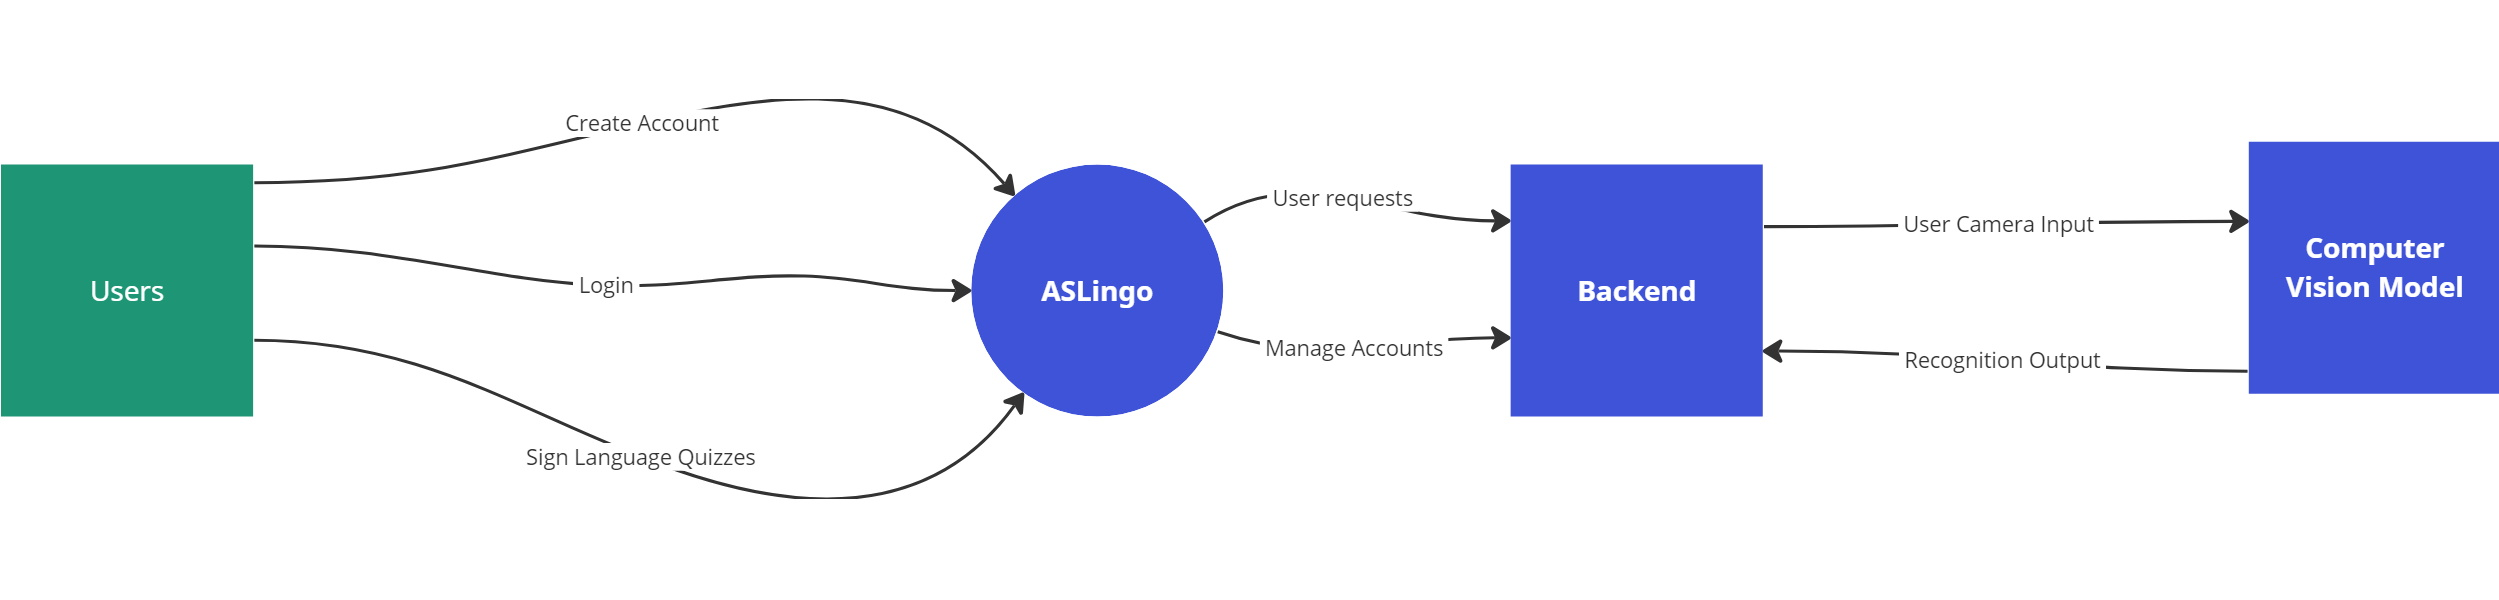
\includegraphics[scale=0.25]{context-diagram}

\subsubsection{Work Partitioning}

\begin{table}[H]
  \caption{Work Partitioning}
  \noindent \begin{tabularx}{\textwidth}{|p{0.2\linewidth}|X|X|}
  \hline 
  \textbf{Event} & \textbf{Input and Output} &\textbf{Description}\\
  \hline
  User requests to log in & User ID (INPUT) \newline User Password (INPUT) \newline Login Status (OUTPUT) & User logs into the application, the system determines if login is successful. \\
  \hline
  User requests to log out & User ID (INPUT) \newline Login Status (OUTPUT) & User logs out of the application, system indicates whether log out is successful or not. \\
  \hline
  User requests to start a test & User ID (INPUT) & User starts a test. \\
  \hline
  User inputs signs through webcam & Camera Feed (INPUT) \newline Recognized Sign (OUTPUT) & User inputs sign language hand signs through webcam, the system responds with the corresponding sign output. \\
  \hline
  \end{tabularx}
  \end{table}

\subsubsection{Individual Product Use Cases}

\subsection{Functional Requirements}
 
** see Table 3: Functional Requirements of ASLingo, might need to format this differently \\

\begin{table}[H]
\caption{Functional Requirements of ASLingo}
\noindent \begin{tabular}{| c | p{4cm}| p{5cm}|}
\hline 
\textbf{Requirement No.} & \textbf{Description} &\textbf{Rationale}\\
\hline
FR1 & The system should be able to connect with a camera. & Connecting with a camera is a requirement for providing input to the system for hand sign recognition. \\
\hline
FR2 & The system should be able to recognize American Sign Language hand signs. & Hand sign recognition is a requirement for users to practice what they have been learning. \\
\hline
FR3 & The system should allow users to create an account. & Account creation is a requirement for users to save progression. \\
\hline
FR4 & The system should allow users to sign into their account if it exists. & Account sign-in is a requirement for users to save progression. \\
\hline
FR5 & The system should provide a diagnostic quiz for new users. & A diagnostic quiz is a requirement for determining the current skill level of the user. \\
\hline
FR6 & The system should provide a progression-based course for ASL. & A progression-based course is a requirement for ensuring users are taught ASL in a comprehensive manner. \\
\hline
FR7 & The system should save user progress. & Saving user progress is a requirement for ensuring the user follows the progression-based course. \\
\hline
FR8 & The system should allow users to access the program via a web application (functional or a constraint?) & \\
\hline
FR9 & The system should be able to communicate to the user if they have answered the prompt correctly. & \\ 
\hline
FR10 & The system should notify the user of any potential errors that may arise during camera recognition. & \\
\bottomrule
\end{tabular}
\end{table}

\section{Non-Functional Requirements}

\subsection{Look and Feel Requirements}

\begin{table}[H]
\caption{Look and Feel Non-Functional Requirements}
\noindent \begin{tabular}{| c | p{3cm}| p{3cm}| p{3cm}|}
\hline 
\textbf{Requirement No.} & \textbf{Description} & \textbf{Rationale} & \textbf{Fit Criterion}\\
\hline
LFR1 & The system should remind users of similar language learning applications & This will allow users to use the system intuitively if they have knowledge of other learning apps. & Ask a sample of users to rate how familiar/easy to use it is compared to other language learning apps. \\
\hline
LFR2 & The system should show the user how much progress they have made in their learning schedule. & The user should be able to gain feedback from the system about how much they learned. & \\
% (level system, progress bar, score after a quiz etc.) 
\hline
LFR3 & The system should clearly show the user if they have answered the prompt correctly. & The user should gain feedback about if they are correct with the hand sign they have shown. & \\
\bottomrule
\end{tabular}
\end{table}

\subsection{Usability and Humanity Requirements}

\begin{table}[H]
\caption{Usability and Humanity Non-Functional Requirements}
\noindent \begin{tabular}{| c | p{3cm}| p{3cm}| p{3cm}|}
\hline 
\textbf{Requirement No.} & \textbf{Description} & \textbf{Rationale} & \textbf{Fit Criterion}\\
\hline
UHR1 & The system should be able to be used by people with little to no training. & The system should be able to be used without the need for formal training to make it easier for the average user. & \\
\hline
UHR2 & The system should be able to be used by people who are hard of hearing or deaf, as well as those who are able to hear. & The system should be accessible for all people wanting to learn ASL. & \\
\hline
UHR3 & The system should allow users to personalize their account. & The user should be able to input their name, see their progress etc. & \\
% (avatar, name, progress; personalization)
\bottomrule
\end{tabular}
\end{table}

\subsection{Performance Requirements}

*can change the time/percents shown* \\ 

\begin{table}[H]
\caption{Performance Non-Functional Requirements}
\noindent \begin{tabular}{| c | p{3cm}| p{3cm}| p{3cm}|}
\hline 
\textbf{Requirement No.} & \textbf{Description} & \textbf{Rationale} & \textbf{Fit Criterion}\\
\hline
PR1 & The system should respond to user input quickly. & If a user has to wait too long after an input they may be less engaged. & 95\%? of tests should repond to user input within 1? second. \\
\hline
PR2 & The system should be able to accurately determine the sign shown by the user. & The system must be able to understand what hand signs the user is inputing to ensure they are learning effectively. & The system should accurately determine a hand sign from a user in 95\%? of tests. \\
% is this functional???
\hline
PR3 & The system should be able to host ??? users at one time. & If there are many people who want to learn ASL at the same time they should be able to do so. & \\
\hline
PR4 & The system should allow for new signs to be added over the lifespan of the system. & This will allow the system to expand over time, as well as be able to add in new modern signs. & \\
\hline
PR5 & The system should show the user if the input needs to be adjusted. & The user should know if they need to change their camera angle, lighting etc. for the system to accurately give them proper feedback. & \\
\bottomrule
\end{tabular}
\end{table}

\subsection{Operational and Environmental Requirements}

\begin{table}[H]
\caption{Operational and Environmental Non-Functional Requirements}
\noindent \begin{tabular}{| c | p{3cm}| p{3cm}| p{3cm}|}
\hline 
\textbf{Requirement No.} & \textbf{Description} & \textbf{Rationale} & \textbf{Fit Criterion}\\
\hline
OER1 & The system should be used as a web application on a browser/laptop. & & \\
\hline
OER2 & The system should be able to access a user's camera device. & & \\
\bottomrule
\end{tabular}
\end{table}

\subsection{Maintainability and Support Requirements}

\begin{table}[H]
\caption{Maintainability and Support Non-Functional Requirements}
\noindent \begin{tabular}{| c | p{3cm}| p{3cm}| p{3cm}|}
\hline 
\textbf{Requirement No.} & \textbf{Description} & \textbf{Rationale} & \textbf{Fit Criterion}\\
\hline
MSR1 & The system should be tested regularly to ensure it's functionality and usability. & & \\
\bottomrule
\end{tabular}
\end{table}

%% Maybe the scalability/longevity requirement from performance?

\subsection{Security Requirements}

\begin{table}[H]
\caption{Security Non-Functional Requirements}
\noindent \begin{tabular}{| c | p{3cm}| p{3cm}| p{3cm}|}
\hline 
\textbf{Requirement No.} & \textbf{Description} & \textbf{Rationale} & \textbf{Fit Criterion}\\
\hline
SR1 & The system should allow the user to access their account after creating it. & & \\
\hline
SR2 & The system should ensure that incorrect input to the system is used. & & \\
\hline
SR3 & The system should store user account info securely? or keep user account info private? & & \\
\bottomrule
\end{tabular}
\end{table}

\subsection{Cultural Requirements}

\begin{table}[H]
\caption{Cultural Non-Functional Requirements}
\noindent \begin{tabular}{| c | p{3cm}| p{3cm}| p{3cm}|}
\hline 
\textbf{Requirement No.} & \textbf{Description} & \textbf{Rationale} & \textbf{Fit Criterion}\\
\hline
CR1 & The system should be written in Canadian English and teach users using American Sign Language.  & & \\
\bottomrule
\end{tabular}
\end{table}

\subsection{Legal Requirements}

\begin{table}[H]
\caption{Legal Non-Functional Requirements}
\noindent \begin{tabular}{| c | p{3cm}| p{3cm}| p{3cm}|}
\hline 
\textbf{Requirement No.} & \textbf{Description} & \textbf{Rationale} & \textbf{Fit Criterion}\\
\hline
LR1 & The system should adhere to user privacy laws?  & & \\
\hline
LR2 & The system should not train the model on personal/confidential/illegal data? & & \\
\bottomrule
\end{tabular}
\end{table}

\subsection{Health and Safety Requirements}

\begin{table}[H]
\caption{Health and Safety Non-Functional Requirements}
\noindent \begin{tabular}{| c | p{3cm}| p{3cm}| p{3cm}|}
\hline 
\textbf{Requirement No.} & \textbf{Description} & \textbf{Rationale} & \textbf{Fit Criterion}\\
\hline
HSR1 &  & & \\
\hline
HSR2 & & & \\
\bottomrule
\end{tabular}
\end{table}

\section{Project Issues}

\subsection{Open Issues}
There are currently no open issues with the project at the moment.

\subsection{Off-the-Shelf Solutions}
\begin{enumerate}
    \item The ASL App is a mobile exclusive platform with 2,500+ signs and phrases to teach ASL via short video clips. This app offers 4 packs for free with the basics like the alphabet, numbers, and universal gestures. Paid packs are also available ex. compliments, moods, and social gestures for \$0.99. The app ultimately serves as a mobile hub for common expressions to study and learn wherever you are.
    \item Canadian Hearing Services offer both in-person and virtual educational ASL courses for a variety of experience levels. These courses educate via teacher instruction, role play, videos, and work books. A variety of other public, private, and educational institutes offer similar courses and instructional content.
    \item Duolingo is a popular mobile application that provides language courses for many languages from across the world, with 50+ million monthly active users. The app utilizes gamification to encourage consistent user progress and interest. Majority of the courses are based on testing users on vocabulary and grammar via reading, listening, and speaking problems which increase in difficulty as users progress. Its courses are well developed through research and accord with global language standards, such as the Common European Framework of Reference for Languages (CEFR).
\end{enumerate}

\subsection{New Problems}
There are currently no new problems.

\subsection{Tasks}
\begin{itemize}
    \item 
    \item Development should follow the agile methodology, with emphasis on different aspects of the project: frontend, backend, and computer vision.
\end{itemize}

\subsection{Migration to the New Product}
Not applicable for our project.

\subsection{Risks}

\begin{enumerate}
    \item The primary risk of this product is the potential for error when trying to analyze and recognize a user's sign to give feedback or determine if their form is correct. This could cause users to improperly learn signs and hinder their learning.
\end{enumerate}

\subsection{Costs}
\begin{enumerate}
    \item Website domain - TBA
    \item App hosting platform - TBA
    \item Database - TBA
\end{enumerate}

\subsection{User Documentation and Training}
The system and it's interface design should be intuitive enough to learn how to use the app.

Possible user documentation to be supplied with the product can include a glossary for numbers and the alphabet, for example. 

SHOULD PROBABLY ADD SOMETHING ELSE!

\subsection{Waiting Room}
\begin{enumerate}
    \item The system should provide different courses for learners of varying skill level.
    \item The system should teach other common sign languages.
\end{enumerate}

\subsection{Ideas for Solutions}

N/A

\bibliographystyle{plainnat}

\bibliography{SRS}

\newpage

\section{Appendix}

This section has been added to the Volere template.  This is where you can place
additional information.

\subsection{Symbolic Parameters}

The definition of the requirements will likely call for SYMBOLIC\_CONSTANTS.
Their values are defined in this section for easy maintenance.

\section{Appendix --- Reflection}

The information in this section will be used to evaluate the team members on the
graduate attribute of Lifelong Learning.  Please answer the following questions:

\begin{enumerate}
  \item Which of the courses you have taken, or are currently taking, will help
  your team to be successful with your capstone project.
  \item What knowledge and skills will the team collectively need to acquire to
  successfully complete this capstone project?  Examples of possible knowledge
  to acquire include domain specific knowledge from the domain of your
  application, or software engineering knowledge, mechatronics knowledge or
  computer science knowledge.  Skills may be related to technology, or writing,
  or presentation, or team management, etc.  You should look to identify at
  least one item for each team member.
  \item For each of the knowledge areas and skills identified in the previous
  question, what are at least two approaches to acquiring the knowledge or
  mastering the skill?  Of the identified approaches, which will each team
  member pursue, and why did they make this choice?
\end{enumerate}


\end{document}